\begin{figure}[H]
  \centering
  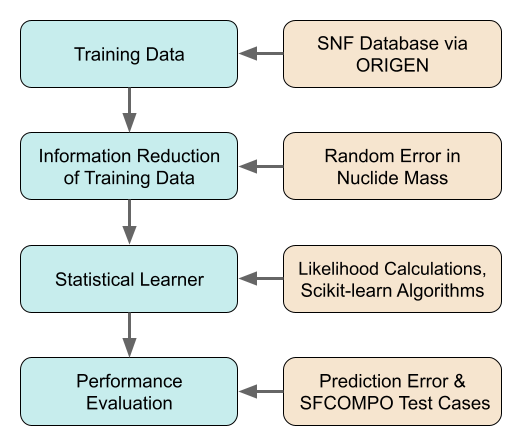
\includegraphics[width=0.7\linewidth]{./chapters/exp1/methodology1.png}
  \caption{First portion of the flowchart from Figure \ref{fig:method} being 
           described in this section.}
\end{figure}

Of interest to an entity trying to create a weapon is partially irradiated fuel
if they have plutonium separations capabilities or any radioactive substance in
the case of a dirty bomb. Thus, this work focuses on \gls{SNF} from commercial
power reactors. Ideally, a large enough database of \gls{SNF} nuclide assays
would be able to be used for this work. Since that does not exist, the 
database will be simulated via \gls{ORIGEN-ARP} \cite{origen, origenarp}.  

\subsection{Simulation Fidelity}
\label{sec:fidelity}

Nuclear fuel cycle studies involve tracking the material flow of nuclear fuel.
This can be anywhere from mining to waste management, or focus on a process
step in between. Fuel cycle studies are not necessarily nuclear-specific. For
example, they can be used to evaluate economic predictions, environmental
impact, transportation planning, etc.  In order to draw conclusions from these
studies, it is common to use a nuclear fuel cycle simulator that tracks the
quantities of interest. These allow the comparison of different fuel types,
reactor technologies, material processing steps, etc. 

There are simplifications researchers need to make in order to experiment in a
controlled way. Fuel cycle simulators, built for a specific needs, must remove
complicating factors that are less relevant to the study.  For example, one
tool might be suited well to large-scale systems analysis with little nuclear
physics included in the models, and another might focus on detailed isotopics
within a system to track plutonium.

Because a large portion of a nuclear forensics investigation relies on
measuring isotopics, this work used \gls{ORIGEN} \cite{origen}, which is a part
of the \gls{SCALE} 6.2 modeling and simulation suite of computational tools
developed for nuclear design and safety \cite{scale}. \gls{ORIGEN} was chosen
for its physically detailed models of activation, depletion, and decay.
Specifically, the ARP module of the code was used: \gls{ORIGEN-ARP}
\cite{origenarp}.

\gls{ORIGEN} calculates time-dependent nuclide concentrations (or quantities
derived from these) that result from activation and depletion calculations. The
physics (i.e., neutron transport and decay) calculations are carried out in
other \gls{SCALE} modules that solve the depletion equations.  This generates
libraries for \gls{ORIGEN} that include the probabilities of reaction (i.e.,
cross sections) for the system.

To obtain an \gls{SNF} recipe from a reactor simulation, \gls{ORIGEN} uses the
desired input power generation with the cross section library to calculate a
flux, the resulting depletion, and the end composition (i.e., isotopic recipes
or nuclide vectors).  Another output is decay; the composition is computed
using decay equations with nuclear data \cite{endf}. These compositions provide
source terms for other calculations, such as decay emission spectra from
neutrons, alpha particles, beta particles, and gamma rays. Other derived
quantities like activity, decay heat, or radiological hazard factors are also
an option.

\gls{ORIGEN-ARP} allows users to access a wider range of simulations by
interpolating between the pre-calculated libraries instead of creating new
libraries.  It is known to be validated for \gls{LWR} \gls{SNF}
\cite{lwr_valid}. Additionally, recycled \gls{SNF} in the form of mixed oxide
fuel has been benchmarked for the relevant reactors \cite{mox_valid}.  Through
\gls{ORIGEN}, given an initial material composition, some reactor operation
parameters, and a reactor type, one can quickly perform many different nuclear
reactor simulations and obtain \gls{SNF} recipes.

\todo[inline]{This section needs more information about ORIGEN-ARP validation
and maybe some nuclides that are known to perform poorly from ARP sims. Can
show a generic example from one of my sources, and or an example of trying to
match an ORIGEN-ARP simulation to an SFCOMPO entry. It is important to inform
that this training set as ground truth is not perfect truth, for some nuclides
more than others. The goal is to explain the ARP validation without getting
too deep.  This tool was necessary for the 500k training set. The prediction
performance will be impacted by the poorly simulated nucs, so it may be
worthwhile to note which ones have consistently large sim errors (unless this
involves getting too deep). P.S. did you mention homogenized core above?}

\subsection{Training Set Labels}
\label{sec:snflbls}

\begin{table}[!htb]
  \centering
  \begin{subtable}{\linewidth}
    \centering
    \begin{tabular}{@{}lll@{}}
    \toprule
      \textbf{PWR} & \textbf{BWR}  & \textbf{PHWR} \\ \toprule
      CE14x14      & GE7x7-0       & CANDU19       \\
      W17x17       & Abb8x8-1      & CANDU28       \\
      S18x18       & Atrium10x10-9 & CANDU37       \\
      BW15x15      & SVEA64-1      &               \\
      VVER440      &               &               \\ \bottomrule
    \end{tabular}
    \caption{\gls{ORIGEN} designations for reactor technologies and fuel assembly design.}
    \label{tbl:rxtrtype}
    \vspace*{5mm}
  \end{subtable}
  \begin{subtable}{\linewidth}
    \centering
    \begin{tabular}{@{}llll@{}}
      \toprule
                              & \textbf{PWR}                     & \textbf{BWR}                     & \textbf{PHWR} \\ \toprule
      Power Density [MW/MTU]  & 25, 35, 41                       & 10, 22                           & 2.2, 18, 22   \\
      Burnup [GWd/MTU]        & 2--68                            & 1--68                            & 0.45--12.6    \\
      Moderator Density [g/cc]& 0.71                             & \{0.1, 0.3, 0.5, 0.7\}           & 0.84          \\
      Enrichment [\% U235]    & \{0.5, 1.5, 2, 3, 4, 5\}         & \{0.5, 1.5, 2, 3, 4, 5\}         & 0.711         \\
      Cooling Time [days]     & \multicolumn{3}{c}{\{0--6000\} in 100-day steps}                                    \\ \bottomrule
    \end{tabular}
    \caption{Simulation parameters for \gls{ORIGEN} input files.}
    \label{tbl:rxtrparam}
  \end{subtable}%
  \caption{Training set database design and parameters for \gls{ORIGEN} input files.}
  \label{tbl:train}
\end{table}

The design of the training set is dependent on a number of factors.  First, it
must have a sufficient number of burnup sets and time since irradiation steps
to provide robust prediction. This is decided upon by maximizing the steps for
both parameters, while balancing the computational limitations of a large
training set. Through previous experience, an approximate limit would be around
$1e6$ database entries for the specific calculations in this work and employing
reasonable computational limitations.

Secondly, the training set must represent what exists in the real world. This
was accomplished by studying the spread of parameters in the \gls{SFCOMPO}
database \cite{sfcompo}.  To ensure this, a variety of reactor types and
assembly designs were included, listed in Table \ref{tbl:rxtrtype}. Table
\ref{tbl:rxtrparam} lists the rest of the simulation inputs. These include not
only the labels of prediction interest, \gls{U235} enrichment, burnup, and time
since irradiation, but also other important simulation input parameters such as
the reactor power density and the moderator density.  (Water is both the
moderator and coolant in all simulated reactor types.)

\begin{figure}[!hbt]
  \makebox[\textwidth][c]{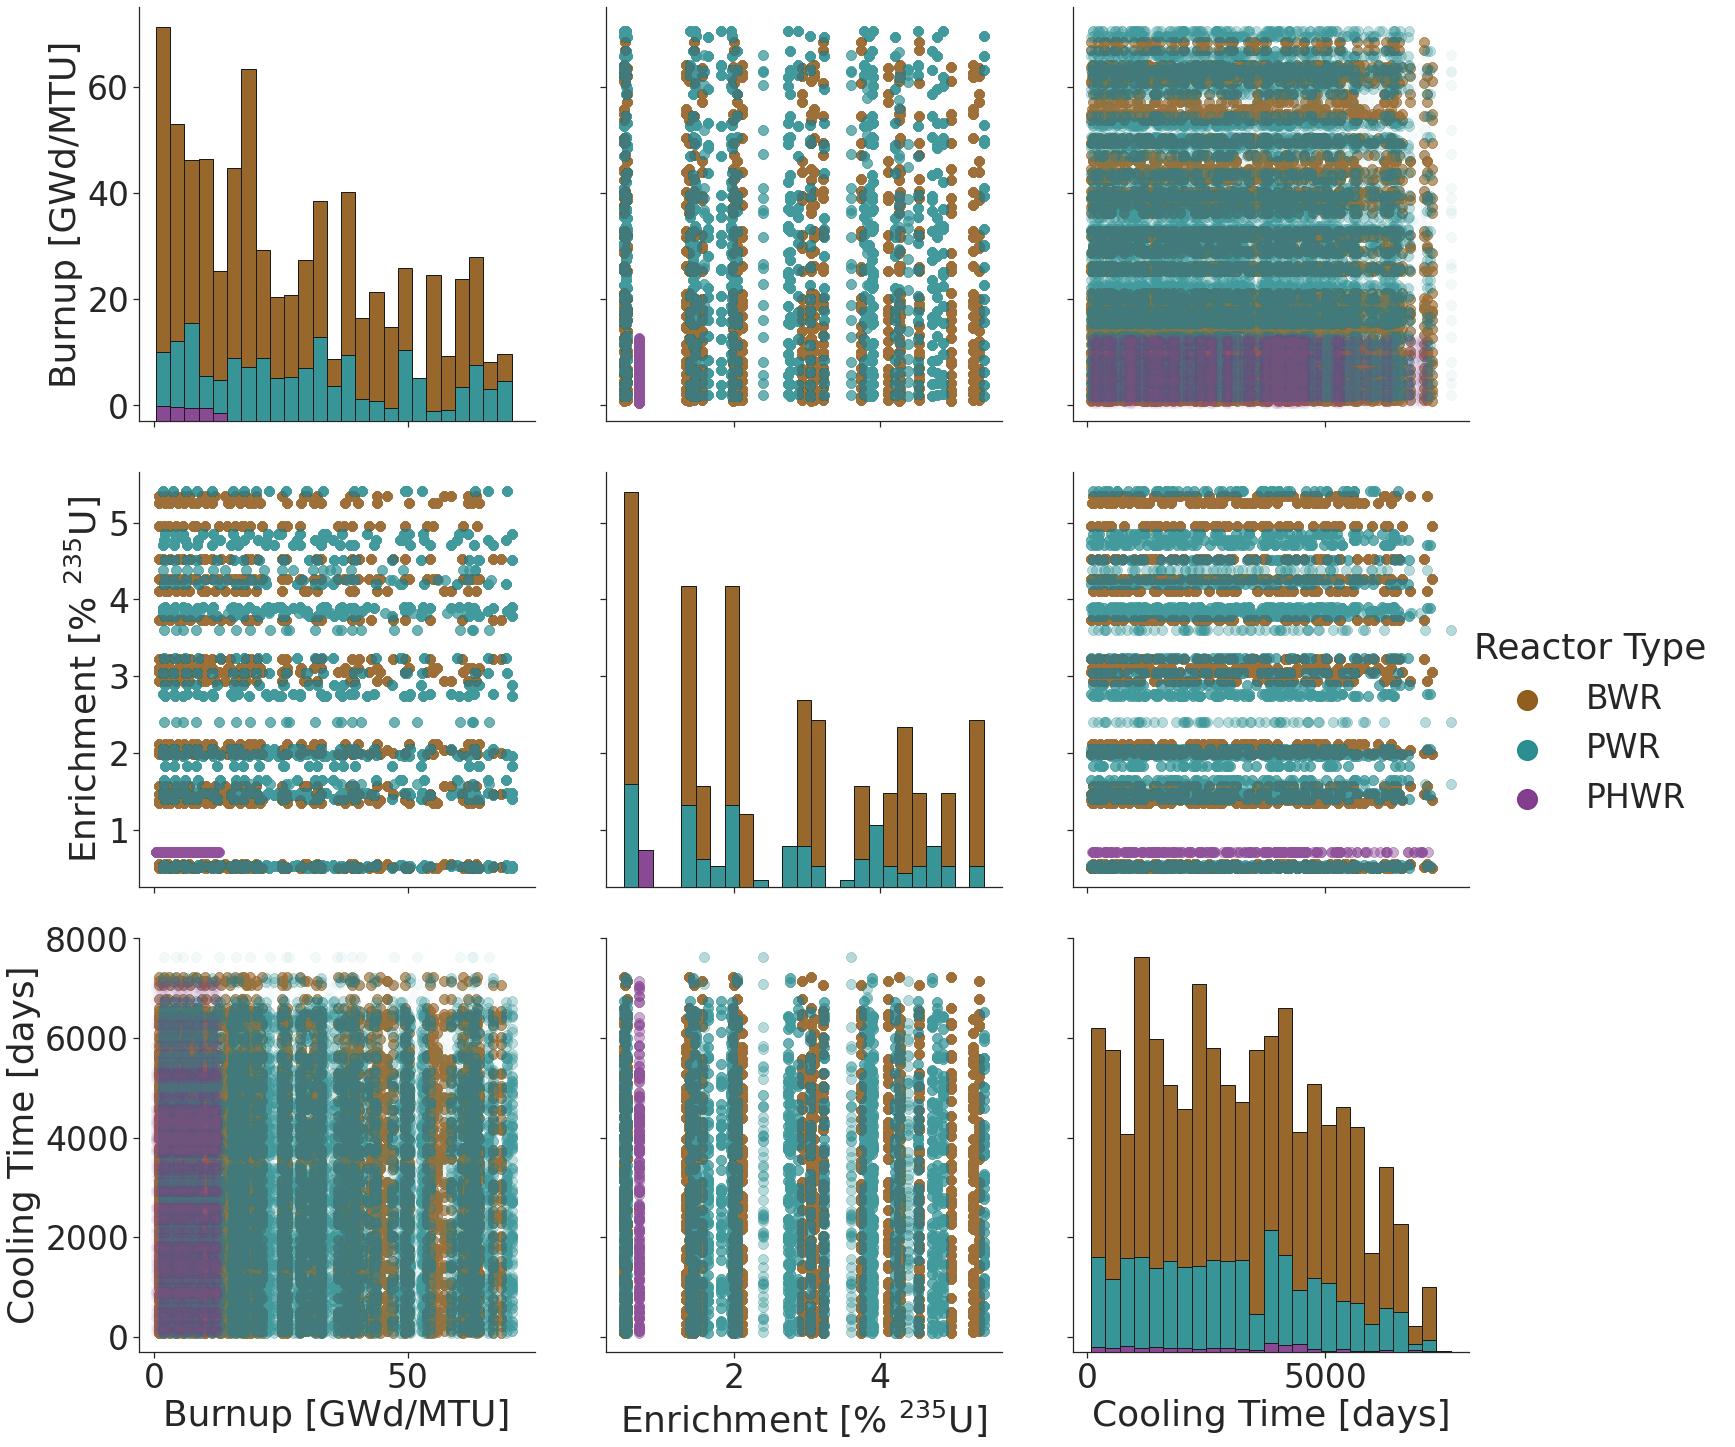
\includegraphics[width=\linewidth]{./chapters/exp1/histogram_scatter_trainset_viz.png}}
  \caption{A combination of histograms and scatter plots to visualize the 
           distribution of prediction labels in the training set.}
  \label{fig:trainhist}
  \todo[inline]{fix the histogram figure, this is a placeholder}
\end{figure}

The third factor influencing database design is ensuring ideal \gls{ML}
algorithm performance.  As mentioned in Section \ref{sec:errs}, many algorithms
are developed with the assumption that the training set will be
\acrfull{i.i.d.}.  This is important so that the model does not overvalue or
overfit a certain area in the training space. With the training set design,
there are predetermined values for enrichment, burnup, and time since
irradiation.  While there are $21-28$ burnup steps (depending on the reactor
type) and 61 cooling time steps, there are only 6 values for enrichment. This
creates the risk that the algorithm will end up being unable to generalize
outside of those discrete values. Therefore, the burnup steps and time steps
are perturbed randomly in a range that is $\pm10\%$ and $\pm30\%$ from the
originally defined values, respectively.  The enrichment also gets perturbed by
$\pm10\%$, and not more because the cross-section libraries in \gls{ORIGEN-ARP}
are pre-calculated for those enrichment values, so deviating too far from them
would result in inaccurate \gls{SNF} simulations. The power densities and
moderator densities were kept at the values defined in Table
\ref{tbl:rxtrparam}.  The resulting training set is $450240$ (or $4.5e5$)
entries.  Figure \ref{fig:trainhist} visualizes the somewhat even distribution
of the burnup and cooling time parameters, and shows the lack of even
distribution of the enrichment parameter through a combination of scatter plots
and histograms.  Note that there are many more \gls{BWR}s present in the
histograms because of the multiple moderator densities simulated (see Table
\ref{tbl:rxtrparam})

\subsection{Training Set Features}
\label{sec:snffeats}

The other design decision regarding the training set is related to
which nuclides to track, i.e., the features.  For this experiment, nuclide
masses are necessary, and the most common measurements in \gls{SFCOMPO} guide
the list of nuclides tracked.  

The set of training features of 29 nuclide masses listed in Table
\ref{tbl:nucmass} was designed with the following reasons in mind.  First, the
units in mass is to represent the scenario of "perfect knowledge", where a full
assay is done via mass spectrometry techniques.  Second, this is to have the
training set units convertable to those present in the external, real-world
test set: the \gls{SFCOMPO} database.  The \gls{ORIGEN} simulations output the
nuclide masses in $grams$, and they are converted to the units of
\textit{milligrams per gram of initial uranium}, $mg/gU_i$, when the models are
externally tested against \gls{SFCOMPO}. Lastly, the 29 nuclides chosen were
based on the presence of measurements in \gls{SFCOMPO}, where these were
present in at least 100 of the samples in the database.  The external test set
is described in more detail in Section \ref{sec:sfcompo}.

\begin{table}[!htb]
  \centering
  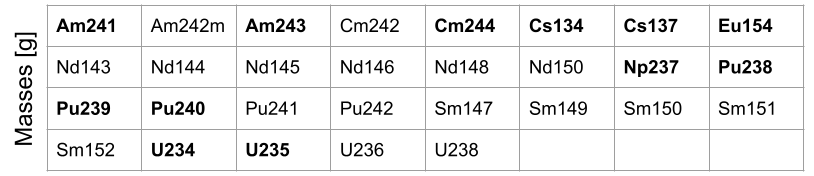
\includegraphics[width=\linewidth]{./chapters/exp1/nucmass_feats.png}
  \caption{Set of features saved for the first experiment, nuclide masses 
           measured in $grams$. The bold nuclide masses overlap with the 
           nuclides in \ref{tbl:nucacts}.}
  \label{tbl:nucmass}
\end{table}

